\documentclass{article}
\usepackage[T1]{fontenc}
\usepackage[MeX]{polski}
\usepackage[english]{babel}
\usepackage[utf8x]{inputenc}
\usepackage{multicol}
\usepackage[pdftex]{graphicx}

\setlength{\oddsidemargin}{-0.25in}
\setlength{\textwidth}{7in}
\setlength{\topmargin}{-.75in} 
\setlength{\textheight}{9.2in} 
\renewcommand{\baselinestretch}{1.5}
\date{}
\title{Zasady prawidłowego żywienia}
\author{Filip Leśkiewicz}
\begin{document}
\maketitle
\renewcommand{\contentsname}{Spis treści}
\renewcommand{\refname}{Bibliografia}
\tableofcontents
\newpage
\section{Zapotrzebowanie kaloryczne}
\subsection{Ogólne zapotrzebowanie}
Ogólnie przyjęte normy dziennego zapotrzebowania kalorycznego to:
\begin {itemize}
\item Dla kobiet:
	\begin {itemize}
	\item od 19. do 50. roku życia: 2200 kcal
	\item powyżej 50. roku życia: 1900 kcal
	\end {itemize}
\item Dla mężczyzn:
	\begin {itemize}
	\item od 19. do 50. roku życia: 2900 kcal
	\item powyżej 50. roku życia: 2300 kcal
	\end {itemize}
\end {itemize}
\subsection{Obliczanie BMR}
BMR (ang. Basal Metabolic Rate) to nic innego jak wyrażona w kaloriach ilość energii jaka jest potrzebna naszemu organizmowi aby utrzymać aktualną masę ciała. Sposobów na jej obliczanie jest wiele, zalecane jest jednak użycie wzoru Harrisa i Benedicta. 
\subsubsection{BMR dla mężczyzn}
Dla mężczyzn wzór na BMR\footnote{M - masa ciała (w kg), W - wzrost (w cm), L -wiek} przyjmuje postać:
$$66,47 + 13,7*M + 5,0*W - 6,76*L$$ \label{bmrm}
\subsubsection{BMR dla kobiet}
Dla kobiet natomiast wygląda on następująco:
$$655,1 + 9,567*M + 1,85*W - 4,68*L$$ \label{bmrk}
\newpage
\subsection{PAL - Physical Activity Level}
Do możliwie najdokładniejszego obliczenia dziennego zapotrzebowania kalorycznego wymagane jest jeszcze poznanie naszej wartości wskaźnika PAL. Jest ona uzależniona od poziomu aktywności fizycznej. Nie musimy wykonywać skomplikowanych obliczeń, wystarczy skorzystać z tabeli poniżej.

\begin{center}
\begin{tabular}{|c|c|c|}
\hline
Aktywność & Ilość ćwiczeń / spacerów & Wartość PAL \\
\hline \hline 
Nieaktywny & Siedzący tryb życia & 1.2 \\ 
\hline 
Słabo aktywny & Spacery i ćwiczenia 1-2 razy w tygodniu & 1.3 \\ 
\hline 
Średnio aktywny & Amatorskie ćwiczenia 2-3 razy w tygodniu & 1.4 \\
\hline
Aktywny & Ciężkie ćwiczenia minimum 3 razy w tygodniu & 1.5 \\
\hline
Mocno aktywny & Cięzkie ćwiczenia codziennie & 1.7 \\
\hline
\end{tabular} \label{pal}
\end{center}

\subsection{Nasze dzienne zapotrzebowanie kaloryczne}
Po użyciu wzorów \ref{bmrm} i \ref{bmrk} oraz odczytaniu z tabeli \ref{pal} odpowiedniej wartości możemy obliczyć nasze własne zapotrzebowanie na kalorie w ciągu jednej doby. W tym celu musimy już tylko pomnożyć otrzymane wartości, czyli wykonać działanie:
$$BMR * PAL$$
Wynik, który otrzymamy to nasze zapotrzebowanie w ciągu 24 godzin. Rzecz jasna, nie powinniśmy jeść byle czego, dlatego też pomocna będzie chociażby piramida ukazana w dalszej części (rysunek \ref{piramid}).

\subsubsection{Modyfikacje w celu stracenia lub przybrania na wadze}
Chcąc stracić na wadze, należy pomnożyć wynik powyższego działania przez 0,85, co spowoduje utratę tkanki tłuszczowej średnio o 0,5 kg tygodniowo. \\
W drugą zaś stronę, jeśli chcemy nabrać masy, należy pomnożyć wynik przez 1,2, co w połączeniu z treningiem oporowym na siłowni możemy przybrać od 0,25 do 0,5 kg miesięcznie.

\section{Co jeść, a czego unikać?}
\subsection{Najczęstsze błędy żywieniowe}
Popełniamy wiele błędów żywieniowych, a o istnieniu niektórych nie mamy nawet świadomości. Wiążą się one zarówno z niedoborem lub nadmiarem spożywanych pokarmów, jak i z nieodpowiednim stylem życia. Najczęściej popełniane z nich to:
\begin{enumerate}
\item Dieta źle zbilansowana pod względem jakościowym (nieodpowiednia jakość wybieranych produktów i częstość ich spożycia) i ilościowym (nieodpowiednia do wieku, płci, aktywności fizycznej i wykonywanej pracy wartość kaloryczna pożywienia oraz niewłaściwe ilości składników odżywczych dostarczanych w pożywieniu oraz nieodpowiednie ich proporcje)
\item Niejedzenie śniadania
\item Nieregularne spożywanie posiłków
\item Spożywanie głównego posiłku wieczorem
\item Podjadanie między posiłkami
\item Codzienne jedzenie słodyczy i/lub tłustych, słonych przekąsek
\item Spożywanie zbyt małej ilości warzyw i płynów
\item Niekontrolowanie jakości spożywanych posiłków (np. nieczytanie etykiet na produktach żywnościowych, nieurozmaicenie posiłków i diety)
\item Uspokajanie się jedzeniem, jedzenie w chwili stresu
\item Robienie zakupów wtedy, kiedy jest się głodnym
\end{enumerate}

\subsection{Podstawowe zmiany w diecie}
Zdrowe odżywianie polega na regularnym dostarczaniu organizmowi wszystkich niezbędnych składników odżywczych w odpowiednich ilościach i proporcjach, lecz nie ma jednoznacznej, wyczerpującej odpowiedzi na temat tego, co powinniśmy jeść, a czego nie. Istnieje mnóstwo odrębnych zdań, jednakże z pewnością można polepszyć swoją dietę stosując się do poniższych reguł:

\begin{enumerate}
\item Spożywaj duże ilości warzyw \newline
Warzywa zawierają mnóstwo korzystnych dla organizmu składników, dlatego powinny być podstawą każdej zdrowej diety. Są nieocenionym źródłem witamin, błonnika pokarmowego i fitozwiązków.
\item Jedz 5 posiłków dziennie \newline
Najważniejsze aby rozpocząć swój dzień od zdrowego i sycącego śniadania. Pozwoli to na zwiększenie wydajności Twojego organizmu i zapobiegnie spożycia nadmiaru kalorii w drugiej części dnia. Kolejne regularne posiłki co 3-4 godziny ustabilizują poziom glukozy we krwi i przyspieszą Twój metabolizm. Jedząc w ten sposób zapewnisz sobie mnóstwo energii przez cały dzień, uchronisz się przed napadami głodu i ciągłym zmęczeniem.
\item Zadbaj o różnorodność \newline
Postaraj się, aby w Twoim dziennym jadłospisie znalazły się artykuły zakwalifikowane do wszystkich grup produktów spożywczych. Wyróżniamy sześć takich grup – produkty zbożowe (pieczywo, kasze, makarony), mleko i jego przetwory (kefir, sery, jogurty, maślanki), warzywa i owoce. Kolejną całą grupę stanowią mięso, ryby i ich przetwory oraz jaja. Do osobnej grupy należą tłuszcze jadalne, czyli oleje roślinne i tłuszcze zwierzęce (masło, łój, smalec). Ostatnią grupą produktów są cukier i wyroby cukiernicze, których spożycie należy zdecydowanie ograniczać.
\item Unikaj wysoko przetworzonych i sztucznych produktów \newline
Unikaj wszelkich fast foodów oraz gotowych dań dostępnych w sklepach. Te wysoce przetworzone produkty nie niosą ze sobą nic dobrego – zawierają masę konserwantów i wzmacniaczy smaku i zapachu (np. aspartam, syrop glukozowo-fruktozowy czy  glutaminian sodu). Do tego charakteryzują się wysoką zawartością tłuszczu i soli, których nadmiar nie wpływa korzystnie na zdrowie. Żywność przetworzona cechuje się również niską, bądź nawet zerową zawartością witamin i składników mineralnych.
\item Nawadniaj swój organizm \newline
Woda spełnia liczne funkcje w naszym organizmie, bierze udział w wielu procesach oraz jest odpowiedzialna za transport substancji odżywczych. Spożycie płynów przez osobę dorosłą powinno kształtować się na poziomie 1,5 – 2 litrów każdego dnia, co łącznie z wodą zawartą w żywności daje około 3 – 3,5 litra dziennie. Skąd taka ilość? Otóż codziennie w procesie oddychania, poprzez układ moczowy, a także z kałem i potem tracimy średnio 2,6 litra wody. Straty wody są jeszcze większe w gorące i wietrzne dni lub w trakcie intensywnego wysiłku fizycznego. Aby organizm mógł w pełni sprawnie funkcjonować każdy ubytek płynu musi być na bieżąco uzupełniany.
\item Unikaj sklepowych słodyczy \newline
Wyroby cukiernicze są źródłem jedynie pustych kalorii (cukier, biała mąka, tłuszcz utwardzony), tak więc dostarczają organizmowi wyłącznie dużej ilości energii, której nadwyżka magazynowana jest w postaci tkanki tłuszczowej. Sklepowe słodycze nie zawierają praktycznie żadnych składników odżywczych. Nadmierne spożycie cukrów prostych może prowadzić do rozwoju nadwagi, próchnicy zębów, a także zaburzeń poziomu glukozy we krwi, a w efekcie cukrzycy. Dlatego należy ograniczać jak najbardziej spożycie słodyczy i wyrobów cukierniczych lub wybierać te z naturalnymi słodzikami, np. ze stewią.
\item Ogranicz korzystanie z soli \newline
Zgodnie z zaleceniami WHO dzienne spożycie chlorku sodu powinno wynosić 5 gram (mała łyżeczka). Okazuje się, że przeciętne spożycie soli w Polsce wynosi aż 15 gram na osobę na dzień! Wynika to z faktu, iż sól występuje w produktach spożywczych jako naturalny składnik, a także dodawana jest do żywności w czasie jej przemysłowego przetwarzania. Duże ilości chlorku sodu używa się w trakcie przygotowywania potraw – na co mamy już bezpośredni wpływ. W związku z tym staraj się nie solić dopóki maksymalnie nie doprawisz dania innymi przyprawami. Unikaj nadmiernego spożycia produktów wędzonych, konserwowych i wysoko przetworzonych.
\item Zamień smażenie na pieczenie \newline
Wszyscy lubimy smażyć – w końcu to jeden z najszybszych sposobów obróbki termicznej popularnych produktów (szczególnie mięsa). Jednak szybko wcale nie znaczy zdrowo!
Jedna łyżka oleju to aż 90 pustych, absolutnie zbędnych kalorii. Zastanów się, ile takich łyżek dodałeś ostatnio smażąc coś na patelni?
Podczas smażenia powstają silnie rakotwórcze związki. Im bardziej „przypalona” jest skórka, tym jest ich więcej.
Większość osób nie umie smażyć poprawnie i nie wie z jakich olejów korzystać oraz jakie są ich temperatury dymienia.
Najprostszym rozwiązaniem wszystkich tych problemów jest zamiana smażenia na pieczenie lub ograniczenie smażenia do minimum.
\item Ogranicz spożycie mięsa \newline
Korzyści wynikające z jedzenia dużych ilości mięsa są bardzo małe w porównaniu do szkód, jakie mogą wyrządzić. Mowa tu przede wszystkim o zwiększeniu ryzyka rozwoju zaburzeń lipidowych i miażdżycy, niektórych nowotworów, chorób układu sercowo – naczyniowego czy przewlekłego zakwaszenia organizmu. W Polsce mięso spożywamy bardzo często pod postacią MOM (mięso oddzielone mechanicznie) i niskiej jakości przetworów co jest szczególnie niebezpieczne dla naszego zdrowia. Oczywiście nie musisz od razu przerzucać się na wegetarianizm. Jeżeli bardzo lubisz mięso i nie wyobrażasz sobie bez niego życia, zwyczajnie jedz je rzadziej i wybieraj tylko chude, wysokiej jakości wyroby.
\end{enumerate}

\subsection{Zdrowe, bezpieczne produkty}
Jest wiele produktów, które możesz jeść bez obaw (oczywiście przy zachowaniu umiaru i równowagi). Pozwolą Ci one na przyrządzanie wielu różnorodnych potraw, co pomoże w trzymaniu się zasad zdrowego żywienia. Niektóre z nich to: 
\begin{multicols}{2}
\begin{itemize}
\item Soczewica 
\item Soja
\item Groch (połówki)
\item Ciecierzyca
\item Fasola 
\item Kukurydza konserwowa
\item Pomidory w puszce
\item Mąka razowa 
\item Mąka graham
\item Mąka kukurydziana
\item Makaron pełnoziarnisty
\item Ryż brązowy
\item Kasza gryczana
\item Kasza jaglana
\item Płatki owsiane
\item Olej rzepakowy
\item Oliwa z oliwek
\item Orzechy włoskie
\item Orzechy laskowe
\item Nasiona słonecznika
\item Pestki dyni
\item Sezam
\item Suszone śliwki
\item Rodzynki
\item Cynamon
\item Bazylia (świeża roślina)
\item Mięta (świeża roślina)
\item Gorzka czekolada
\end{itemize}
\end{multicols} 
\section{Wskaźnik masy ciała}
Wskaźnik masy ciała (ang. Body Mass Index (BMI) to współczynnik powstały przez podzielenie masy ciała podanej w kilogramach przez kwadrat wysokości podanej w metrach. Klasyfikacja (zakres wartości) wskaźnika BMI została opracowana wyłącznie dla dorosłych i nie może być stosowana u dzieci. \\
Oznaczanie wskaźnika masy ciała ma znaczenie w ocenie zagrożenia chorobami związanymi z nadwagą i otyłością, np. cukrzycą, chorobą niedokrwienną serca, miażdżycą. Podwyższona wartość BMI związana jest ze zwiększonym ryzykiem wystąpienia takich chorób.
\subsection{Jak obliczać BMI}
Do obliczenia naszego BMI musimy wykorzystać wzór:
$$BMI = \frac{M}{W^2}$$ \\
Gdzie oznaczenia literowe są takie same, jak w przypadku wzorów \ref{bmrm} i \ref{bmrk}.

\subsection{Zakresy wartości}
Poszerzona klasyfikacja wartości BMI to:
\begin{center}
\begin{tabular}{|c|c|}
\hline
Wartość & Znaczenie \\
\hline 
\hline
$< 16,0$ & Wygłodzenie \\ 
\hline 
16,0–16,99 & Wychudzenie \\
\hline 
17,0–18,49 & Niedowaga \\
\hline
18,5–24,99 & Wartość prawidłowa \\
\hline
25,0–29,99 & Nadwaga \\
\hline
30,0–34,99 & I stopień otyłości \\
\hline
35,0–39,99 & II stopień otyłości \\
\hline
$≥ 40,0$ & III stopień otyłości \\
\hline

\end{tabular} \label{bmi}
\end{center}
Jak łatwo się domyśleć, nasz wskaźnik powinien mieścić się w przedziale wartości prawidłowej. Jeśli wartość ta wykracza w jedną, bądź drugą stronę poza przedział, wskazana jest modyfikacja diety i trybu życia - pomocne może okazać się zasięgnięcie opinii dietetyka.
\newpage

\section{Odwrócona piramida żywieniowa}
Piramida ta jest kierowana do osób zdrowych w celu zachowania dobrego stanu zdrowia. Jest to jak najprostsze ogólne przedstawienie kompleksowej idei żywienia. Jak ją czytać? Otóż im wyższe piętro w piramidzie, tym rzadziej i mniej należy spożywać danych produktów. Skrupulatna dieta zgodnie z poniższymi wytycznymi da nam szansę na zdrowe i długie życie oraz dłuższe zachowanie sprawności intelektualnej i fizycznej.
\newline
\begin{figure}[h]
\begin{center}
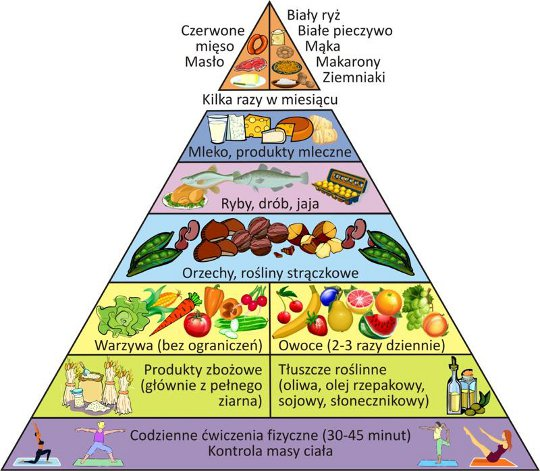
\includegraphics[width=0.8\textwidth]{piramida.jpg} \label{piramid}
\end{center}
\end{figure}
\newpage
\begin{thebibliography}{4}
\bibitem{bib_1} Anna Bogacka, ,,Zdrowie na talerzu", wyd. Studio Astropsychologii, 2008
\bibitem{bib_2} Michael Pollan, ,,Jak jeść. Przewodnik konsumenta", wyd. Poradnia K., 2010
\bibitem{bib_3} Zdrowe odżywianie - blog z pysznymi i szybkimi przepisami na zdrowe jedzenie <http://zdrowe-odzywianie-przepisy.blogspot.com/>
\bibitem{bib_4} CoJesc.Net - blog o zdrowym odżywianiu, jedzeniu i dietetyce <http://cojesc.net/>
\bibitem{bib_5} abcZdrowie.pl - portal o zdrowiu i zdrowym stylu życia <https://portal.abczdrowie.pl/>
\end{thebibliography}

\end{document}
